\documentclass{paper}
\usepackage{mathrsfs,amsmath, wasysym, geometry, pstricks, graphicx, type1cm, lettrine, float, fancyhdr}
\usepackage[super]{nth}
\geometry{a4paper}
\usepackage{algorithm}

\usepackage{algpseudocode}
\usepackage{graphicx}
\usepackage{microtype}
\usepackage{pdfpages}
\usepackage[framed,numbered,autolinebreaks,useliterate]{mcode}
\PassOptionsToPackage{hyphens}{url}\usepackage{hyperref}\usepackage{hyperref}

\newcommand{\HRule}{\rule{\linewidth}{0.5mm}}
\usepackage{listings}
\definecolor{mygreen}{rgb}{0,0.6,0}
\definecolor{mygray}{rgb}{0.8,0.8,0.8}
\definecolor{mymauve}{rgb}{0.58,0,0.82}

\pagestyle{fancy}
\lhead{ENB440 - \emph{Milestone 1}}
\lfoot{ENB440 \emph{Group 06}}

\begin{document}
\newpage
\begin{titlepage}
\begin{center}

\textsc{\LARGE ENB440 RF Techniques and Modern Applications}\\[0.75cm]

\begin{figure}[H]
\centering

\includegraphics[width=0.2\textwidth]{IMG/QUT} \\[0.75cm]
\end{figure}

\textsc{\Large ENB440 - Filter Design}\\[0.5cm]

% Title
\HRule \\[0.4cm]
{ \huge \bfseries Design Milestone 1 \\[0.4cm] }

\HRule \\[1.5cm]



\begin{minipage}{0.4\textwidth}
\begin{flushleft} \large
Grant \textsc{Kennedy} \\
\emph{n8566712}\\
Blake \textsc{Fuller} \\
\emph{n8598819}\\
\end{flushleft}
\end{minipage}
\begin{minipage}{0.4\textwidth}
\begin{flushright} \large


\emph{Group 06}\\
\end{flushright}
\end{minipage}

\vfill

% Bottom of the page
{\large \today}
\end{center}
\end{titlepage}

\section*{Executive Summary}
In this report a 70$\Omega$ microstrip is characterised through mathematic calculation, then designed and modeled within the CST Design Suite software environment.\\

Transmission and reflection characteristics are first calculated in section ~\ref{sec:handcalcs} in terms of ABCD parameters, from which the geometry of the system is calculated. The microstrip geometries are then independently found by using TX-Line software in section ~\ref{sec:tx-line}.\\

CST modeling methods and S parameters are evaluated in section ~\ref{sec:CST}. Passband, return loss and transmission are discussed in terms of the microstrip S parameters.\\

Optimisation within CST is discussed and results are displayed in section ~\ref{sec:optimise}. Conclusions are draw on the exercise and different design methods in section ~\ref{sec:conclusion}.\\

A microstrip design is presented with full analysis of its characteristics.\\ 

\newpage
\tableofcontents

\newpage
\section{Introduction}
This report details the design of a simple 70$\Omega$ microstrip Printed Circuit Board (PCB) using Rogers RO4003C. \\

Circuit characteristics are calculated in three ways:

\begin{enumerate}
	\item Hand calculations
	\item MATLAB calculations
	\item Computer generated results\\
\end{enumerate}

These are compared before modeling the system within the CST software suite.\\
\newpage
\section{Line Impedance Calculations}
\subsection{Hand Calculations}
\label{sec:handcalcs}
First we found the ABCD parameters for the circuit shown in Figure~\ref{fig:theoretical_circuit}. Once found they were converted to scattering parameters.

\begin{figure}[H]
	\centering
	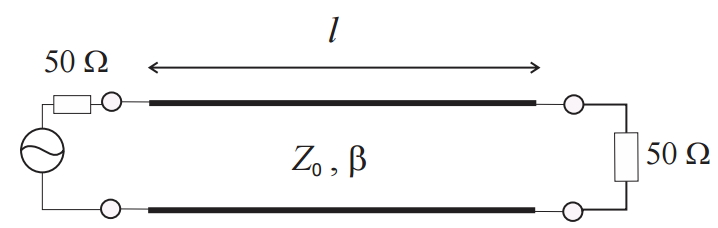
\includegraphics[scale=0.5]{IMG/theoretical_circuit}
	\caption{Theoretical stripline circuit}
	\label{fig:theoretical_circuit}
\end{figure}

This circuit consists of two 50$\Omega$ loads and two sections of transmission line with an electrical length of $\lambda$ and an impedence($Z_0$) of $70\Omega$. The wave number ($\beta$) is given by:
$$\beta = \frac{2\pi}{\lambda}$$
The unsimplified ABCD representation for this circuit is the following:
$$\begin{bmatrix}
A & B\\
C & D
\end{bmatrix} = 
\begin{bmatrix}
1 & 50\\
0 & 1
\end{bmatrix}
\begin{bmatrix}
cos(\beta\l) & j70sin(\beta\l)\\
\frac{jsin(\beta\l)}{70} & cos(\beta\l)
\end{bmatrix}
\begin{bmatrix}
1 & 50\\
0 & 1
\end{bmatrix}
\begin{bmatrix}
cos(\beta\l) & j70sin(\beta\l)\\
\frac{jsin(\beta\l)}{70} & cos(\beta\l)
\end{bmatrix}
$$
As $\beta\l=2\pi$ the sin terms are 0 and the cos terms become 1. The results for the ABCD matrix are as follows:
$$\begin{bmatrix}
A & B\\
C & D
\end{bmatrix} = 
\begin{bmatrix}
1 & 100\\
0 & 1
\end{bmatrix}
$$
The conversion from ABCD to scattering parameters is shown here:
\begin{align}
S_{11} &=\frac{A+B/Z_0-CZ_0-D}{A+B/Z_0+CZ_0+D}\\
S_{11} &=\frac{1+100/70-0-1}{1+100/70+0+1}\\
S_{11} &=\frac{5}{12}\\
&= 20log(S_{11})= -7.6042dB
\end{align}
\begin{align}
S_{12} &= \frac{2(AD-BC)}{A+B/Z_0+CZ_0+D}\\
S_{12} &= \frac{2(1-0)}{1+100/70+0+1}\\
S_{12} &= \frac{7}{12} \\ 
&= 20log(S_{12})= -4.6817dB
\end{align}
\begin{align}
S_{21} &= \frac{2}{A+B/Z_0+CZ_0+D}\\
S_{21} &= \frac{2}{1+100/70+0+1}\\
S_{21} &= \frac{7}{12} \\
&= 20log(S_{21})= -4.6817dB
\end{align}
\begin{align}
S_{22} &= \frac{-A+B/Z_0-CZ_0+D}{A+B/Z_0 +CZ_0+D}\\
S_{22} &= \frac{-1+100/70-0+1}{1+100/70+0+1}\\
S_{22} &= \frac{5}{12} \\
&= 20log(S_{22})= -7.6042dB
\end{align}
\subsection{Matlab Results}
We attempted to replicate the hand calculations in Matlab in order to model the S paramaters over the 2-4 GHz range where length was constant. The code to perform the calculations is noted in the appendix 1 and figure ~\ref{fig:matlab_S} was generated.

\begin{figure}[H]
	\centering
	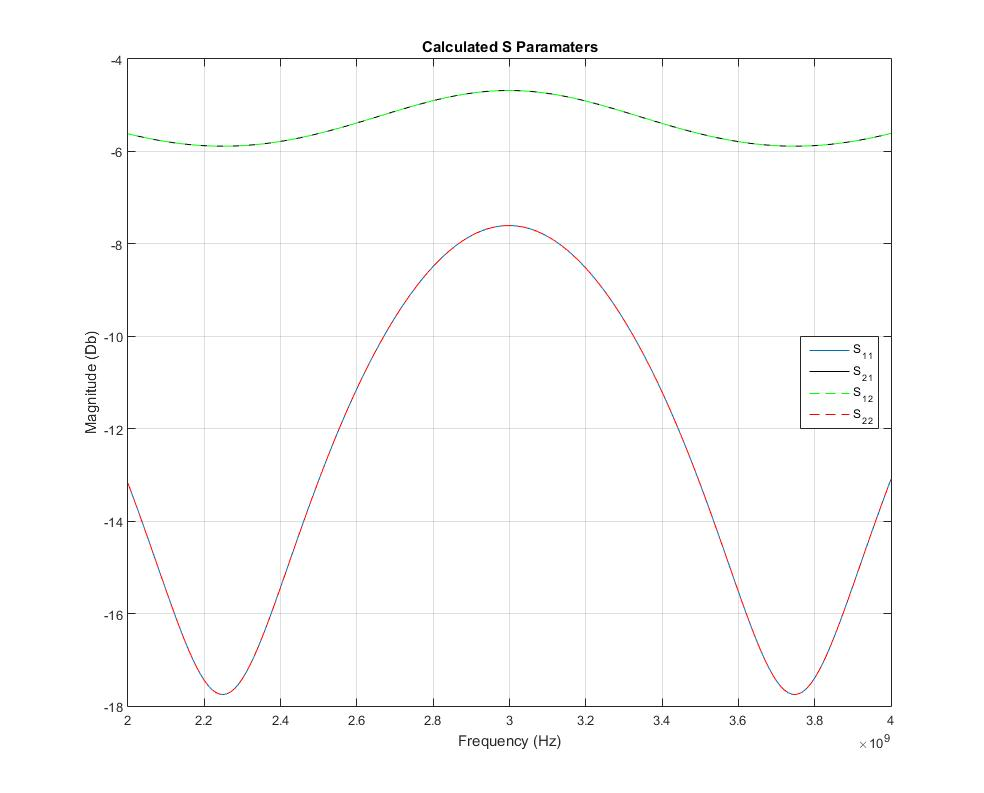
\includegraphics[scale=0.5]{IMG/ideal_sweep}
	\caption{S Paramaters from 2-4 GHz}
	\label{fig:matlab_S}
\end{figure}

This plot did not satisfactorily match our expectations for an ideal sweep of the circuits scattering parameters. This is because it shows the attenuation of reflection decreasing towards the design frequency. Our expectation was for the opposite to happen as is seen in the section on Computer Generated Results.

One reason the difference may have occurred is that the line was modelled in ABCD as:
$$Load->Line->Load->Line$$
where both loads and lines were considered equal. The ground plain would possibly have differences to the copper strip and could very well account for an error. It is reasonable to conclude that the code may be performing an incorrect process to measure the scattering parameters of this system as it is so different to the result in CST. The amount of work required to make this graph alone shows the usefulness of CST for this task.

Figure ~\ref{fig:varying_l} shows the S parameters matching the values from the hand calculations. This is due to the length being changed across the frequency range to stay at 1 wavelength.

\begin{figure}[H]
	\centering
	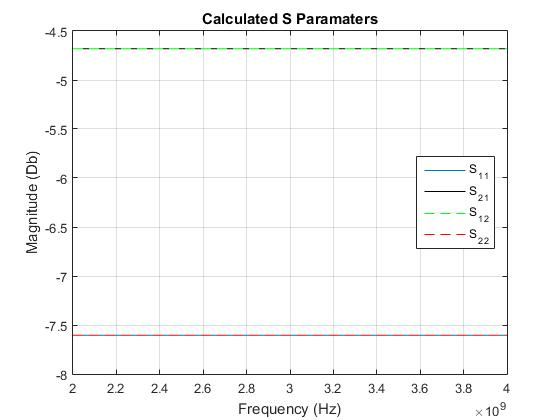
\includegraphics[scale=0.5]{IMG/varying_l}
	\caption{S Paramaters from 2-4 GHz}
	\label{fig:varying_l}
\end{figure}

This exercise has served to highlight the usefulness of CST for modelling this system.


\subsection{Computer Generated Results}
\label{sec:tx-line}
The National Instruments (NI) program TX-Line was used to generate an approximation of the microstrip geometry. The given laminate, impedance, frequency and electrical length information were input and the program output the microstrip width and length. \\

These values can be seen in the TX-Line GUI screenshop in figure ~\ref{fig:txline}  

\begin{figure}[H]
	\centering
	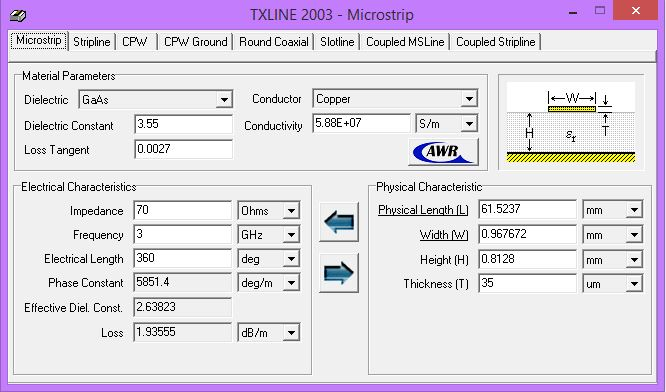
\includegraphics[scale=0.6]{IMG/txline}
	\caption{Screenshot of TX-Line program.}
	\label{fig:txline}
\end{figure}

The following data was found from the results:

\begin{center}
	\begin{tabular}{c|c}
		\hline
		Characteristic & Result\\\hline\hline
		Phase Constant & 0.102126 rad/mm\\\hline
		Physical Length & 61.5237 mm\\	\hline
		Width & 0.967672 mm\\\hline
		Eff. Diel. Const. & 2.63823\\\hline
	\end{tabular}
\end{center}

\newpage
\section{Modeling}
\label{sec:CST}
The microstrip was modeled in CST, with a frequency range of 2GHz to 4GHz and port information defined at 3GHz. The computer generated results found from TX-Line were initially used and resulted in the model that can be seen below in figure ~\ref{fig:stripline1}.\\

\begin{figure}[H]
	\centering
	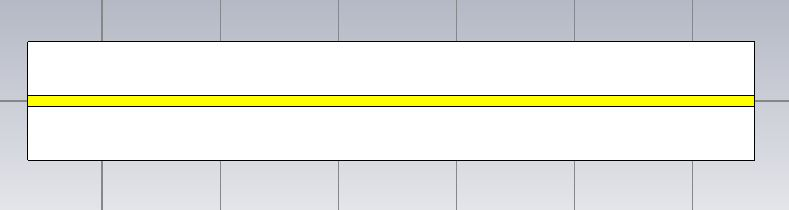
\includegraphics[scale=0.5]{IMG/CSTStripline}
	\caption{CST Microstrip model.}
	\label{fig:stripline1}
\end{figure}

The reflection (S$_{11}$ and S$_{22}$) and transmission S parameters (S$_{21}$ and S$_{12}$) were then found after simulation. These can be seen below in figure ~\ref{fig:s11_s22_s21_s12}.

\begin{figure}[H]
	\centering
	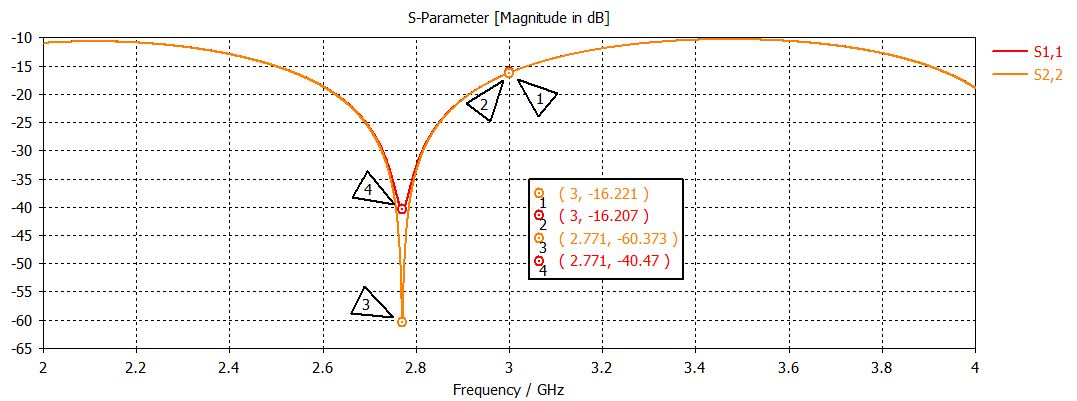
\includegraphics[scale=0.4]{IMG/S11_and_S22}
	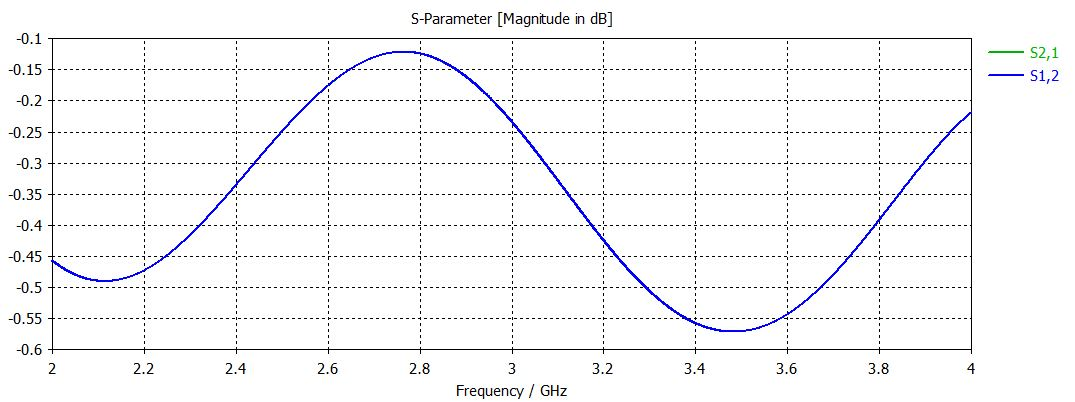
\includegraphics[scale=0.4]{IMG/S21_and_S12}
	\caption{Top: S$_{11}$ and S$_{22}$ parameters - magnitude. Bottom: S$_{21}$ and S$_{12}$ parameters - magnitude.}
	\label{fig:s11_s22_s21_s12}
\end{figure}

It can be seen that the loss of the microstrip along the transmission S parameter $S_{21}$ is 0.239dB. This value is expected - the loss in the copper and dielectric would result in a low loss, especially given the loss tangent of RO4003C being as low as 0.0027.\\

The passband of the system is seen to peak at 2.771GHz with very little loss (passband at -60dB S$_{11}$ and -40dB S$_{22}$). At the specified transmission frequency of 3GHz the reflection of the microstrip is -16dB, causing return losses. The cause of this is the mismatch between the 50$\Omega$ source port and the 70$\Omega$ microstrip.\\

The phase of all S parameters can be seen below in figure ~\ref{fig:s11_s22_s21_s12_phase}.\\

\begin{figure}[H]
	\centering
	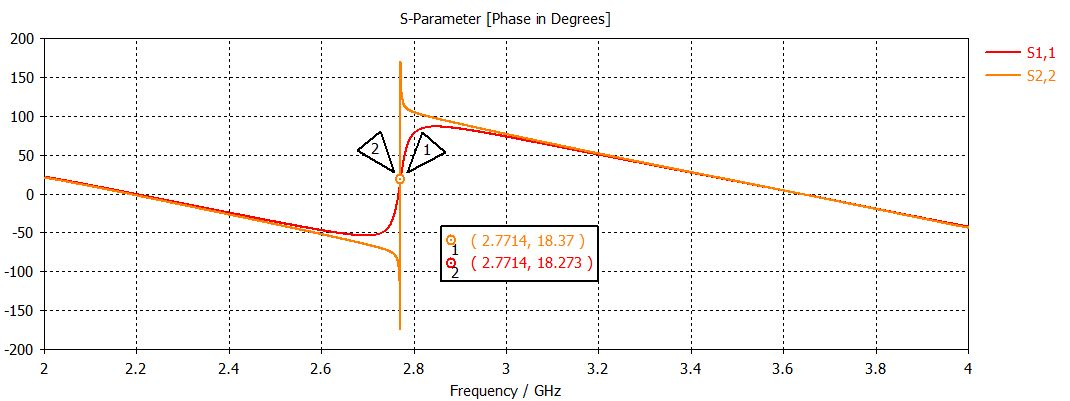
\includegraphics[scale=0.4]{IMG/S11_and_S22_phase}
	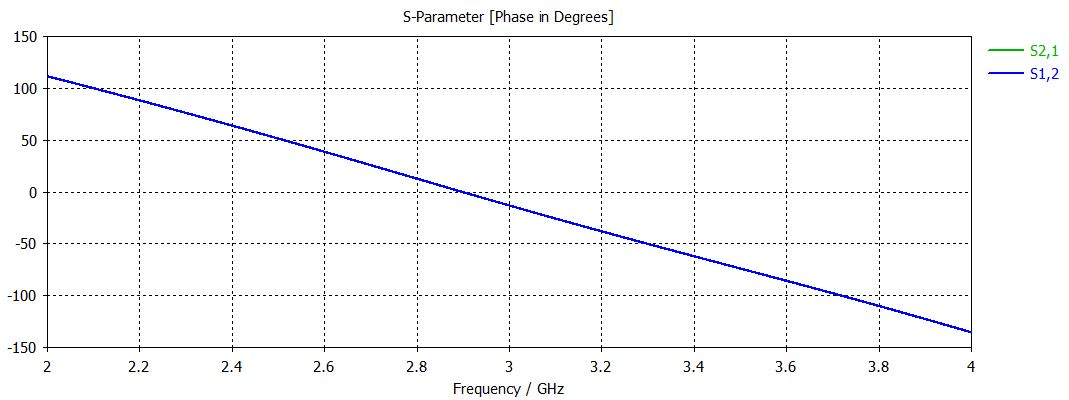
\includegraphics[scale=0.4]{IMG/S21_and_S12_phase}
	\caption{Top: S$_{11}$ and S$_{22}$ parameters - phase. Bottom: S$_{21}$ and S$_{12}$ parameters - phase.}
	\label{fig:s11_s22_s21_s12_phase}
\end{figure}

All S parameter phase plots are linear, as expected. \\

The S$_{11}$ and S$_{22}$ plots have an abnormality at 2.7714GHz, which is caused by the passband peak.\\

The line impedance, as calculated by CST, is seen to be 51$\Omega$, which is noticeably different to the expected value of 70$\Omega$. Initially, all geometries and material parameters were checked to ensure that this value wasn't an issue with the model. After thorough inspection no errors were found with the model.\\

\begin{figure}[H]
	\centering
	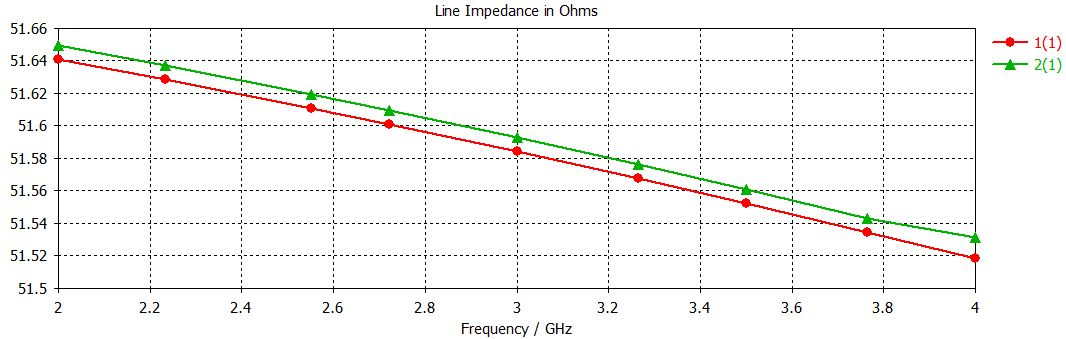
\includegraphics[scale=0.4]{IMG/51ohm}
	\caption{Original line impedance.}
	\label{fig:orig_line_imp}
\end{figure}

\newpage
\subsection{CST Optimiser}
\label{sec:optimise}
The optimiser was used to calculate geometries needed to achieve a line impedance of 70$\Omega$. The goal of modifying the S$_{11}$ parameter was judged as being irrelevant given the system is to be designed with a line impedance of 70$\Omega$ with 50$\Omega$ ports.\\ 

As the electrical length, height of dielectric and copper thickness all couldn't be altered, the microstrip width was chosen as the variable to optimise.\\

After optimisation, the following line impedance was found.\\

\begin{figure}[H]
	\centering
	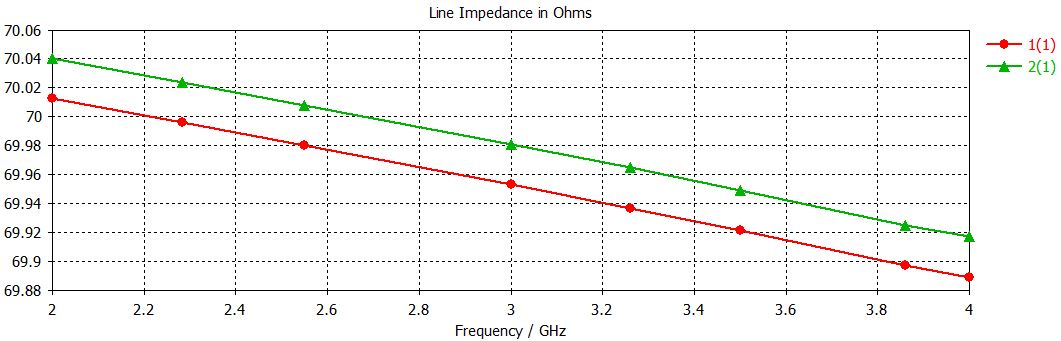
\includegraphics[scale=0.4]{IMG/70ohm}
	\caption{Modified line impedance.}
	\label{fig:mod_line_imp}
\end{figure}

The optimisation software altered the original microstrip width of 0.9676mm to 0.5536mm which resulted in a line impedance of 70$\Omega$. The resulting S$_{11}$ and S$_{22}$ parameters can be seen below. There is no notable different information in the S$_{21}$ and S$_{12}$ parameters.

\begin{figure}[H]
	\centering
	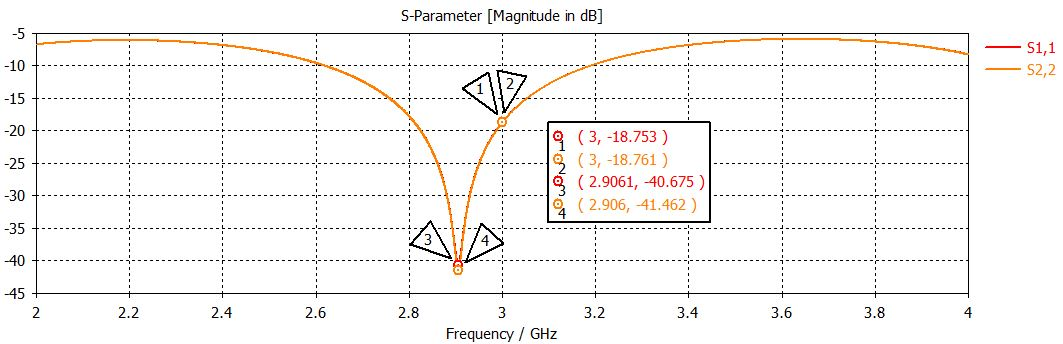
\includegraphics[scale=0.4]{IMG/70ohm_s11_s22}
	\caption{Modified line impedance.}
	\label{fig:mod_line_s11_s22}
\end{figure}

It can be seen that the optimisation method has matched the line impedance to the required impedance. The reflection peak has also moved closer to the operating frequency.

\newpage
\section{Conclusion}
\label{sec:conclusion}
Doing similar calculations in three different ways has been helpful in understanding the processes that go on under the hood of established programs. By calculating the microstrip characteristics manually one can get a feel for how a problem will be solved and whether output values seem realistic. \\

Familiarity with these kinds of processes can also come through many repetitions of using purpose built programs like CST. It allows for rapid iteration and gainful experimentation with differing system geometries. CST also allows for fine tuning of results once they are obtained to make small gains which could mean the difference between meeting specification or not.\\

The hand calculations and MATLAB calculations are less precise methods of calculating S parameters as they don't account for factors such as dielectric and conductor losses. \\

In this way, the first methods of system characterisation are important and very much have their place, but a design suite is needed for full system design.

\newpage
\section{Appendices}
\subsection{MATLAB Script}
\begin{lstlisting}
%% ENB440
clc
clear
close all
%% Q2:

c = 299792458; % Speed of light
f = (2:0.01:4)*10^(9); % 2-4 GHz Sweep
epr = 3.55;             %Given material relative permitivity
w = 0.967672*10^(-3); % Width
d = 0.8128*10^(-3); %Substrate Thickness

% epeff = (epr+1)/2+(epr-1)/2*1/sqrt(1+12*d/w); % Effective permitivity
epeff = 2.6126765618828367;% Calculated Effective Permitivity
lambda = c./f./sqrt(epeff);
l = 4*15.466682984821468*10^-3; % Calculated Length
beta = 2*pi./lambda;

z1 = 50;
z2 = 50;
z0 = 70;
y0 = 1/z0;
ABCD = zeros (2,2,length(f));
for i=1: length(f)
    ABCD(:,:,i) = [1 z1; 0 1]*[cos(beta(i)*l) 1j*z0*sin(beta(i)*l); 1j*y0*sin(beta(i)*l) cos(beta(i)*l)]...
        *[1 z2; 0 1]*[cos(beta(i)*l) 1j*z0*sin(beta(i)*l); 1j*y0*sin(beta(i)*l) cos(beta(i)*l)];
end
A = squeeze(ABCD(1,1,:))';
B = squeeze(ABCD(1,2,:))';
C = squeeze(ABCD(2,1,:))';
D = squeeze(ABCD(2,2,:))';

s11 = 20*log10(((A+B./z0-C*z0-D)./(A+B./z0+C.*z0+D)));
s12 = 20*log10((2*(A.*D-B.*C))./(A+B./z0+C.*z0+D));
s21 = 20*log10((2)./(A+B/z0+C.*z0+D));
s22 = 20*log10((-A+B./z0-C*z0+D)./(A+B./z0+C.*z0+D));

figure();
plot (f,(s11))
hold on
plot (f,(s21),'k')
plot (f,(s12),'g--')
plot (f,(s22),'r--')

legend('S_1_1','S_2_1','S_1_2','S_2_2','location','east')
grid on
title('Calculated S Paramaters');
xlabel('Frequency (Hz)');
ylabel('Magnitude (Db)');
\end{lstlisting}
Appendix 1: MATLAB

\end{document}